\documentclass{article}
\usepackage[utf8]{inputenc}
\usepackage{amsmath,amssymb}
\usepackage{graphicx}
\usepackage{float}
\usepackage{subcaption}
\usepackage{geometry}
\geometry{
    a4paper,
    total={170mm,257mm},
    left=20mm,
    right=20mm,
    top=20mm,
}
\usepackage{listings} % code listings
\lstset{framextopmargin=0pt,frame=lines}
\lstset{
    language=Matlab,
    basicstyle=\footnotesize\ttfamily,
    breaklines=true,
    tabsize=4,
    keepspaces=true,
    columns=flexible,
    % backgroundcolor=\color[gray]{0.9},
    frame=single,
    breaklines=true,%
    morekeywords={matlab2tikz},
    keywordstyle=\color{blue},%
    morekeywords=[2]{1}, keywordstyle=[2]{\color{black}},
    identifierstyle=\color{black},%
    stringstyle=\color{mylilas},
    commentstyle=\color{mygreen},%
    showstringspaces=false,%without this there will be a symbol in the places where there is a space
    numbers=left,
    numberstyle={\tiny \color{black}},% size of the numbers
    numbersep=9pt, % this defines how far the numbers are from the text
    emph=[1]{for,end,break},emphstyle=[1]\color{red}, %some words to emphasise
    %emph=[2]{word1,word2}, emphstyle=[2]{style},
}
\usepackage{color} %red, green, blue, yellow, cyan, magenta, black, white
\definecolor{mygreen}{RGB}{28,172,0} % color values Red, Green, Blue
\definecolor{mylilas}{RGB}{170,55,241}

\title{ENV-541 Sensor Orientation\\Lab 5 - Inertial Navigation in 2D / Realistic Signal}
\author{Michael Spieler}
\date{November 2, 2018}

\begin{document}

\maketitle

\section*{Stochastic error values}


\begin{table}[h]
\centering
\begin{tabular}{llll}
Error type & Notation & Value & Note \\
\hline
\textbf{Gyro} bias (random constant) & $b_G$ & $XXrad/s$ & $1\sigma$ \\
\textbf{Gyro} correlation noise (1st order Gauss-Markov) & $\sigma_{G^{PSD}_{GM1}}$ & $XXrad/s/\sqrt{Hz}$ & PSD level \\
& $1/\beta_G$ & $100s$ & correlation time \\
\textbf{Gyro} random walk (white noise) & $\sigma_{G^{PSD}_{WN}}$  & $XXrad/s/sample$ & PSD level \\
% \hline
\textbf{Accelerometer} bias (random constant) & $b_A$  & $XXm/s^2$ & $1\sigma$ \\
\textbf{Accelerometer} noise (white)  & $\sigma_{G^{PSD}_{WN}}$  & $XXm/s^2/sample$ & PSD level
\end{tabular}
\caption{Stochastic error values in SI units.}
\label{tab:err_val}
\end{table}

\section*{Error plots}
\begin{figure}[H]
    \centering
    \begin{subfigure}[t]{0.49\textwidth}
        \centering
        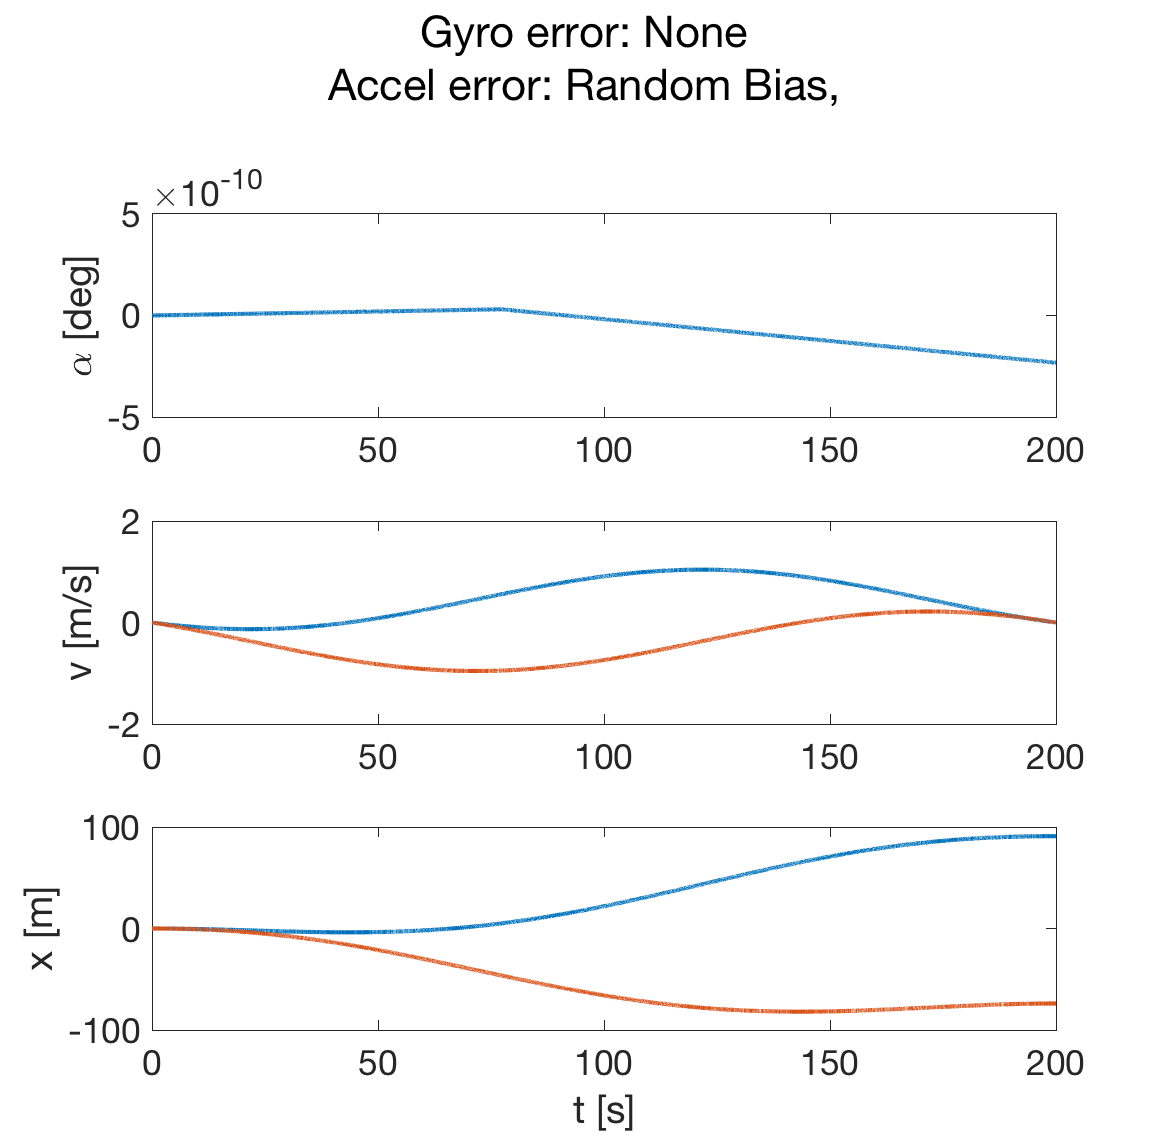
\includegraphics[width=\textwidth]{fig/accel_bc}
        \caption{}
    \end{subfigure}
    ~
    \begin{subfigure}[t]{0.49\textwidth}
        \centering
        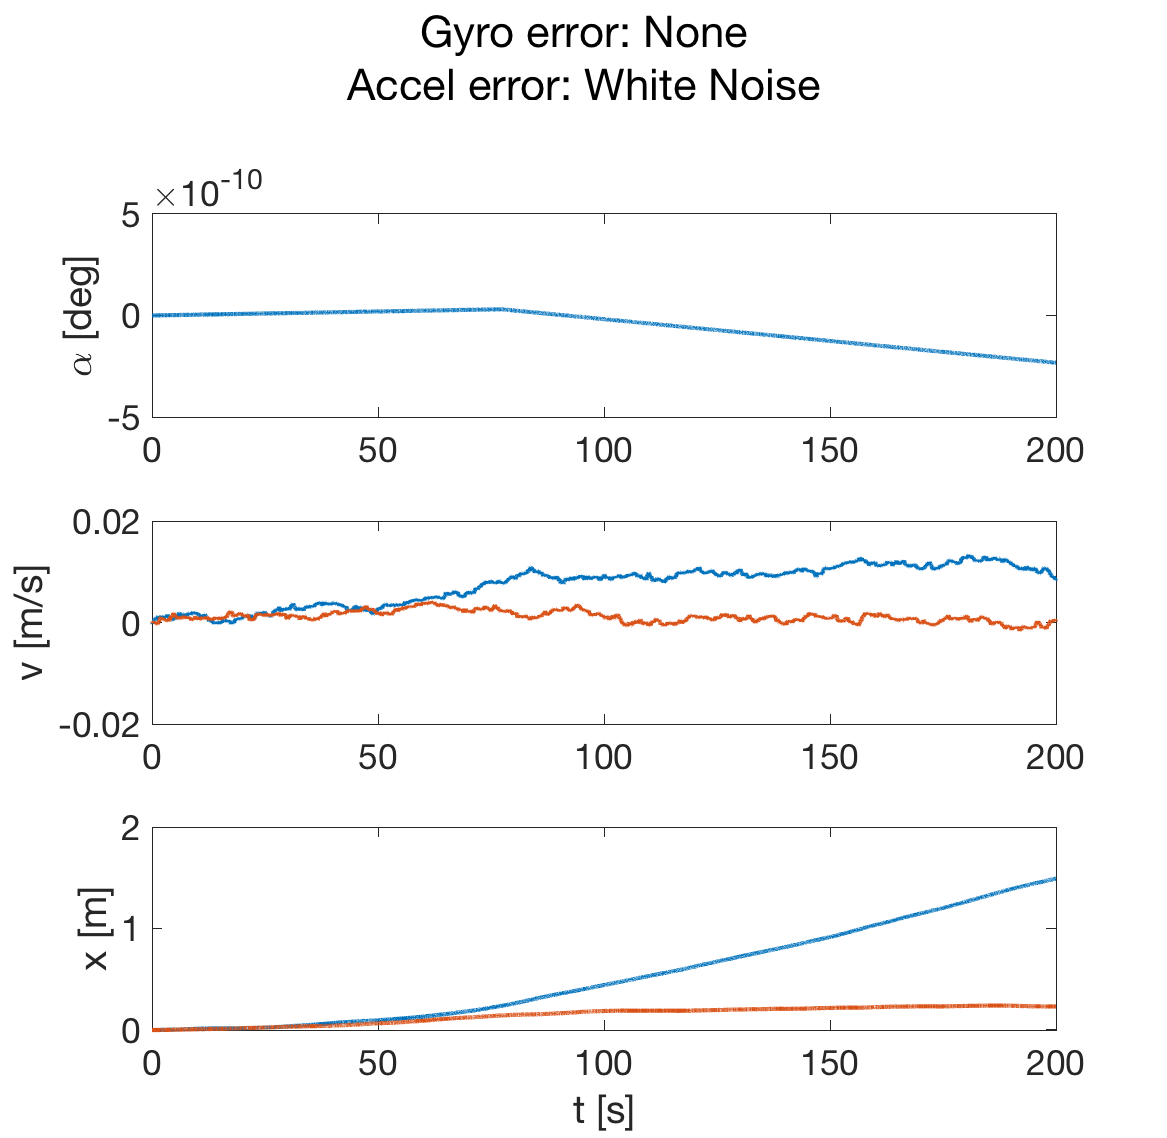
\includegraphics[width=\textwidth]{fig/accel_wn}
        \caption{}
    \end{subfigure}
    \caption{Trajectory errors from accelerometer noise.}
    \label{fig:error_accel_1}
\end{figure}

\begin{figure}[H]
    \centering
    \begin{subfigure}[t]{0.49\textwidth}
        \centering
        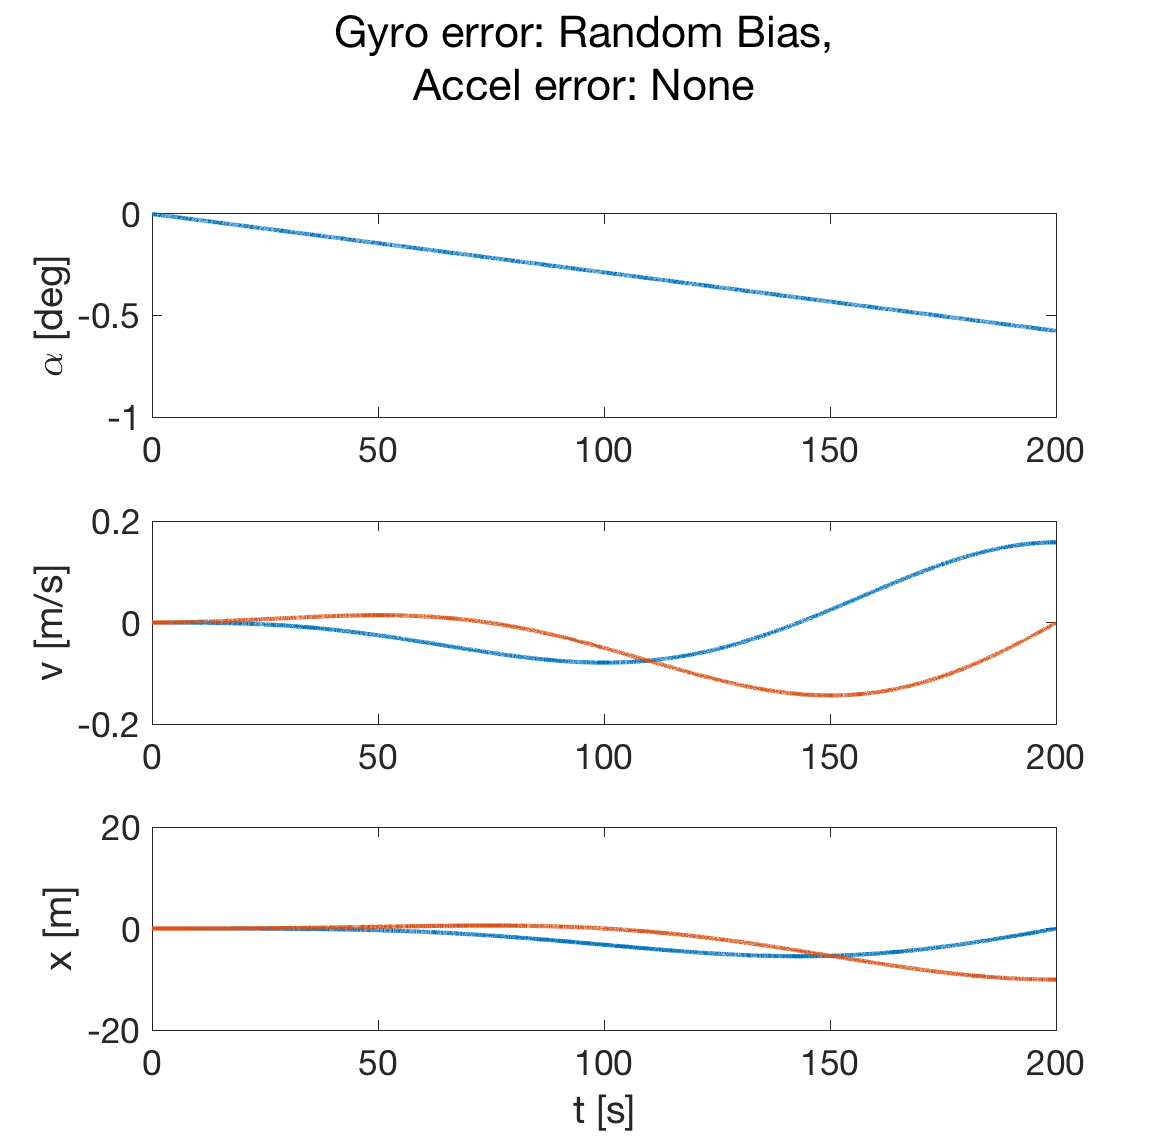
\includegraphics[width=\textwidth]{fig/gyro_bc}
        \caption{}
    \end{subfigure}
    ~
    \begin{subfigure}[t]{0.49\textwidth}
        \centering
        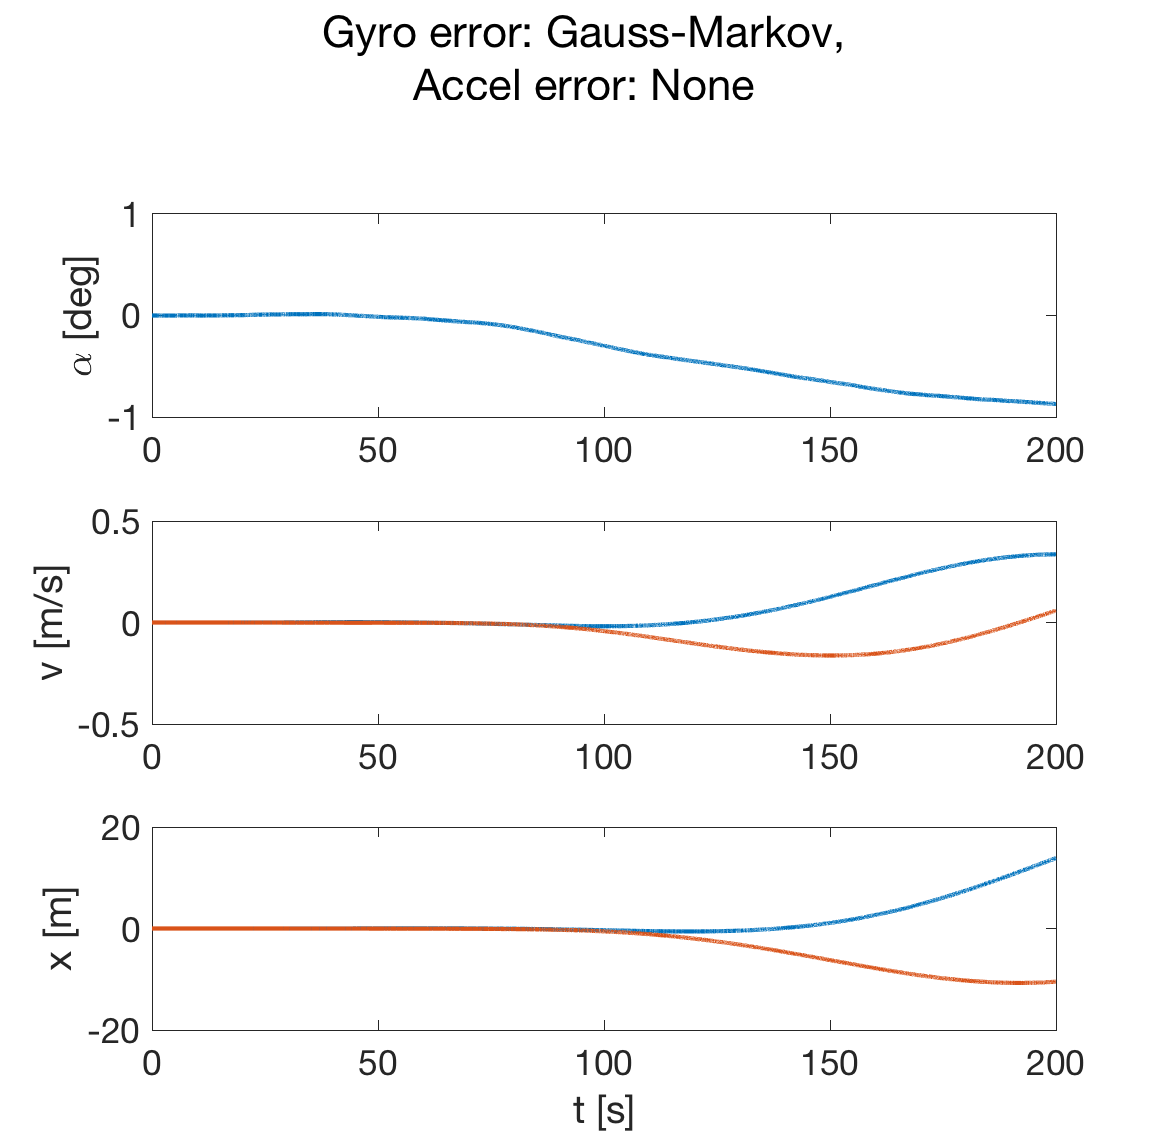
\includegraphics[width=\textwidth]{fig/gyro_gm}
        \caption{}
    \end{subfigure}
    \caption{Trajectory errors from gyro noise}
    \label{fig:error_gyro_1}
\end{figure}

\begin{figure}[H]
    \centering
    \begin{subfigure}[t]{0.49\textwidth}
        \centering
        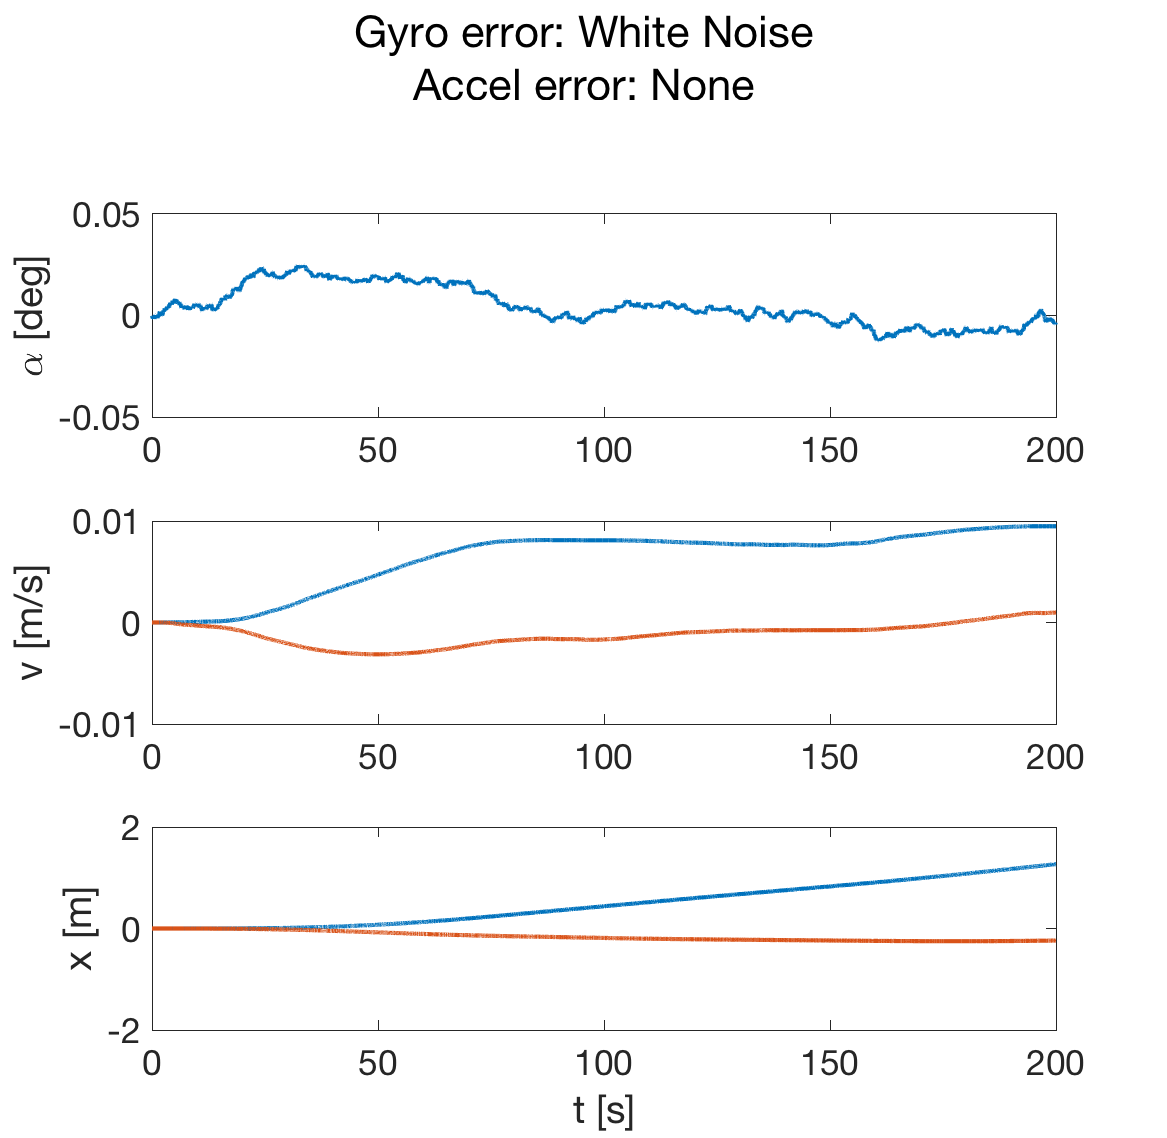
\includegraphics[width=\textwidth]{fig/gyro_wn}
        \caption{}
    \end{subfigure}
    \caption{Trajectory errors at 100Hz sampling rate}
    \label{fig:error_gyro_2}
\end{figure}

% \newpage
\section*{Code}
\lstinputlisting{../lab5.m}

\end{document}
